\documentclass[border=0.2cm]{standalone}
% Required packages and libraries
\usepackage{tikz}
\usetikzlibrary{automata, arrows.meta, positioning}
\begin{document}
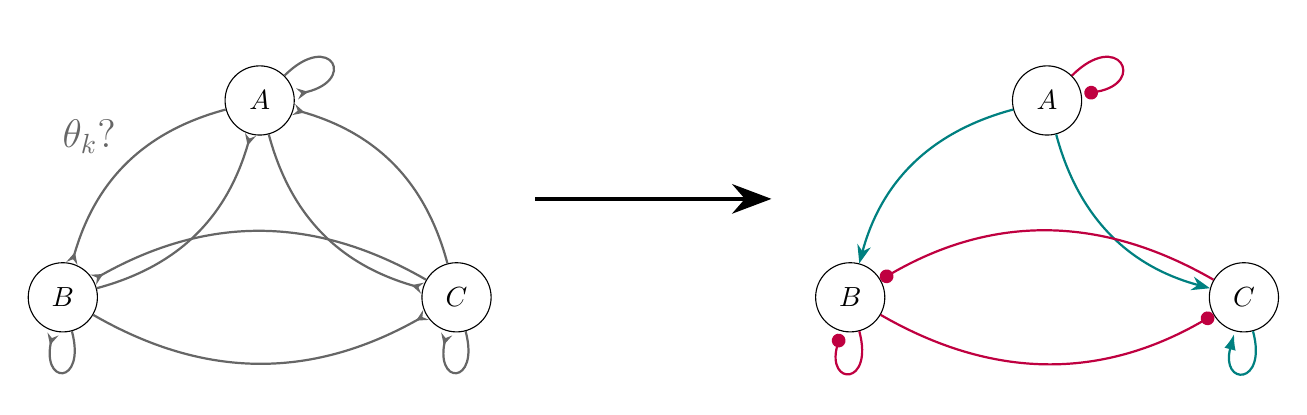
\begin{tikzpicture}
\node (AA) [state] at (2.5,2.5) {$A$};
\node (BB) [state] at (0,0) {$B$};
\node (CC) [state] at (5,0) {$C$};
\node (A) [state] at (12.5,2.5) {$A$};
\node (B) [state] at (10,0) {$B$};
\node (C) [state] at (15,0) {$C$};

\draw[-{Stealth[length=5mm]}, line width=0.5mm] (6,1.25) -- (9,1.25);

%Unknown:
\path [thick,every loop/.append style=-{Latex[length=2mm]},every loop/.append style=-{stealth reversed}]
(AA) edge [in =10, out=45, loop,color=gray!80!black] (AA)
(BB) edge [loop below,color=gray!80!black] ()
(CC) edge [loop below,color=gray!80!black] ()
(AA) edge [bend right, -stealth reversed,color=gray!80!black] (CC)
(AA) edge [bend right, -stealth reversed,color=gray!80!black] node[above left] {\Large $\theta_k$?} (BB)
(BB) edge [bend right, -stealth reversed,color=gray!80!black] (AA)
(BB) edge [bend right, -stealth reversed,color=gray!80!black] (CC)
(CC) edge [bend right, -stealth reversed,color=gray!80!black] (AA)
(CC) edge [bend right, -stealth reversed,color=gray!80!black] (BB)
;

%Activation
\path [-stealth, thick,every loop/.append style=-{Latex[length=2mm]}]
(A) edge [bend right, -Stealth,color=teal] (B)
(A) edge [bend right, -Stealth,color=teal] (C)
(C) edge [loop below,color=teal] ()
;
%Repression:
\path [thick,every loop/.append style=-{Latex[length=2mm]},every loop/.append style=-{Circle}]
(A) edge [in =10, out=45, loop,color=purple] (A)
(B) edge [loop below,color=purple] ()
(C) edge [bend right, -Circle,color=purple] (B)
(B) edge [bend right, -Circle,color=purple] (C)
;


\end{tikzpicture}
\end{document}